\documentclass[a4paper]{report}
\usepackage[utf8]{inputenc}
\usepackage{url}
\usepackage{float}
\usepackage{wrapfig}
\usepackage{graphicx}
\usepackage[toc,page]{appendix}
\graphicspath{ {images/} }
\restylefloat{figure}
\renewcommand*{\thesection}{\arabic{section}}
\renewcommand{\thesubsection}{\thesection(\alph{subsection})}

\begin{document}
\begin{titlepage}
    \begin{center}
        \includegraphics[width=0.7\textwidth]{uol-logo}

        \vspace{5em}

        \Large{COMP390}
        \vspace{1em}
        \Large{\\2020/21}

        \vspace{3em}

        \Large{Generative Adversarial Networks for Terrain Generation}

        \vspace{3em}

        \begin{tabular}{|lp{5.0cm}lll|}
            \hline
                                      &                    &  &   & \\
            \textbf{Student Name:}    & Laura Hulley

            \                         &                    &  &     \\
            \textbf{Student ID:}      & 201277571

            \                         &                    &  &     \\
            \textbf{Supervisor Name:} & Prof Paul Dunne

            \                         &                    &  &     \\
            \hline
        \end{tabular}

        \vspace{3em}

        \LARGE{{\textbf{DEPARTMENT OF\\
                        COMPUTER SCIENCE}}}

        \vspace{2em}

        University of Liverpool\\Liverpool L69 3BX

    \end{center}



\end{titlepage}
\section{Dedication}
\section{AnonTitle}
\section{Abstract}
\section{Contents}
\section{Introduction}

\subsection{Aims and Objectives}
\subsection{Video Game Terrain}
As the video game industry grows, so does the need for more detailed, exciting and extensive terrains. Procedural terrain generation has been an integral part of video games throughout their existence. An early example of such being the entirely ASCII-based 1980 game, Rogue \cite{rogue}. The level maps, treasure and monsters are procedurally generated each time the game is played. Rogue inspired future games and spawned the category of Rogue-like games which now contains hundreds, if not thousands,\footnote{Figure estimated from Steam search results \cite{roguelikeSteam} and the following list \cite{roguebasin_2020}. There is also the assumption that there are unpublished video games developed using rogue-like techniques.} of procedurally generated games.

The response to the demand for more realistic terrain can be seen in the development of the snowboarding game, SSX(2012) \cite{SSX}. This was the first game in the SSX series to use real world terrain data and the response was overwhelmingly positive. While this was impressive in 2012, it would struggle to compete with the infinite, procedurally generated maps of today's games.

While the terrain in Rogue was formed using simple rule based algorithms, more complex algorithms are needed to create terrain that resembles the natural land forms found on earth. Fractal and noise based techniques can generate incredibly realistic terrain without the limitations of real world data. They offer infinite results and more widely customisable terrain but not without their own drawbacks.

\begin{figure}[H]
    \centering
        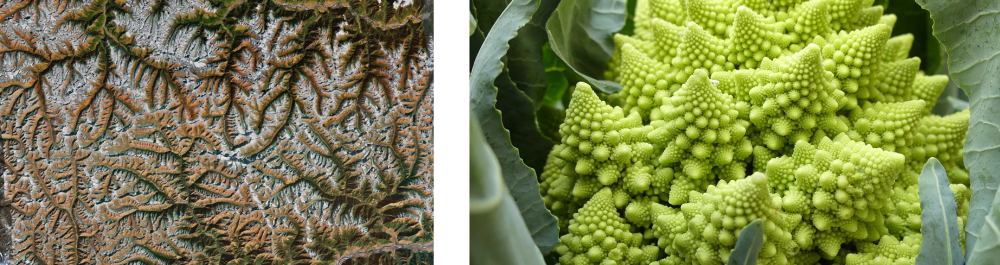
\includegraphics[width=0.9\textwidth]{fractals.png}
        \caption{Shows }
        \label{fig:fractals}
\end{figure}

\paragraph{Fractal Techniques}

Fractals are seen throughout the natural world, from mountains, to rivers, to broccoli (figure \ref{fig:fractals}). Fractals are recursive algorithms that preserve self similarity. In nature, an element of randomness is always present and one algorithm that aims to replicate this is the diamond square algorithm.

The D-Sq algorithm begins with a 2d array, the 4 corners of which are set to some initial values. It then iterates between calculating the midpoint of that square, then the midpoints of the resulting `diamonds'. A diagram of the steps involved is shown in figure \ref{fig:ToDo}. To better understand the algorithm, a simple Python implementation was made which demonstrates the effects of changing the randomness of the algorithm and the resulting `roughness' of the terrain. Figure \ref{fig:ToDo} shows the output of the D-Sq script with varying levels of roughness. Two main criticisms of this technique are the presence of artefacts in the resulting terrain and the unrealistic terrain generated (either too regular or too random)\cite{Dsq}. Figure \ref{fig:ToDo}(a) is an example of the repetitive patterns often generated by this technique. No `mountain' is exactly the same, due to the addition a random value at each iteration, but as a group they can seem unnaturally repetitive. Conversely, with higher levels of roughness or randomness, the mountains can be too steep, sparse and random. Another common problem associated with this technique is the artefacts left behind. Pinches can form between the tiles when the edge values do not line up \cite{ToDo}. 

\paragraph{Combined Techniques}
\subsubsection{Generative Adversarial Networks}
Overall overview
\paragraph{Terrain Generation with GANs}
j
\section{Design and Implementation}
\subsection{Dataset}
\subsection{LandGAN}
\section{Testing and Evaluation}
\section{Conclusion}
\subsection{Further developments}
\appendix
\renewcommand\bibname{References}
\bibliographystyle{IEEEtran}
\bibliography{refs}
\begin{appendices}
\section{Previous Work}
\subsection{Aims}
\begin{enumerate}
    \item Demonstrate the ability of a GAN to produce realistic and efficient\footnote{The definition of what constitutes realistic and efficient in this project is described in section 0.6} terrain elevation and rendering.
    \item Form a discussion that compares the effectiveness of a GAN technique to more traditional algorithmic techniques.
\end{enumerate}
\subsection{Objectives}
\subsubsection{Aim 1}
\begin{enumerate}
\renewcommand{\theenumi}{\alph{enumi}}
    \item Source satellite image and elevation data of the planet that is legally available for educational use.
    \item Source a sufficient amount of training data for the GAN to enable a fair comparison. The definition of a sufficient amount of training data for the discriminator would need to be defined in later stages of the project after initially testing the success of the model.
    \item Define a measure of success for the GAN.
    \item Develop a GAN with the aim of producing results that are indistinguishable by humans from those in the original data set. This objective is a desirable requirement of the model developed, however the closer the model is to reaching this standard, the better we are able to argue the merits of this approach. The process of developing a GAN will also increase my personal understanding of the subject and allow a more informed discussion.
\end{enumerate}
\subsubsection{Aim 2}
\begin{enumerate}
    \renewcommand{\theenumi}{\alph{enumi}}
    \item Outline the main similarities and differences between the use of GANs and traditional approaches to terrain generation.
    \item Form a meaningful argument. As this project is an investigation into how one technique compares to another, there is no bias to have a definite `winner'. To be classified as a meaningful argument, in line with the aforementioned article, this objective would be satisfied by completion of objectives c-f.
    \item Frame of reference: Define the context in which these techniques are being measured. For example, in the intended context of game design, it is worth noting why we would place more weight on the efficiency of the program at the expense of realism.
    \item Grounds for comparison: Explain the rationale behind the choice of terrain generation techniques used as examples in the project.
    \item Clearly define the relationship between the techniques: "Do they extend, corroborate, complicate, contradict, correct, or debate one another?" \cite{Walk:1998}
    \item Form the comparison around a clear organisational scheme.
    \end{enumerate}
\section{Code}
Code here

\begin{figure}[H]
    \centering
        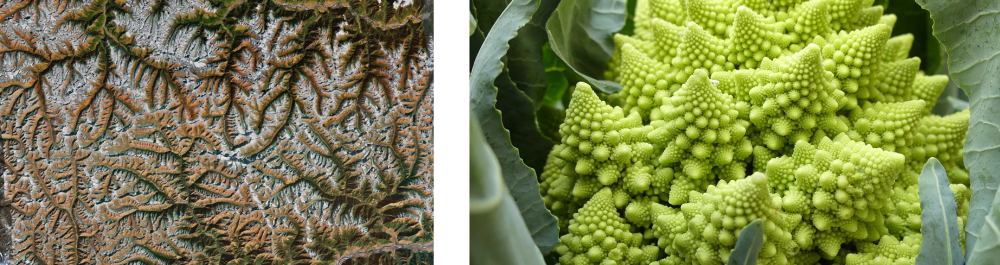
\includegraphics[width=0.9\textwidth]{fractals.png}
        \caption{Shows }
        \label{fig:ToDo}
\end{figure}
\end{appendices}
\end{document}